\newpage

\section{Auswertung}
\subsection{Beobachtung der Aufspaltung}
\subsubsection{Transversale Konfiguration}
\begin{figure}
\centering
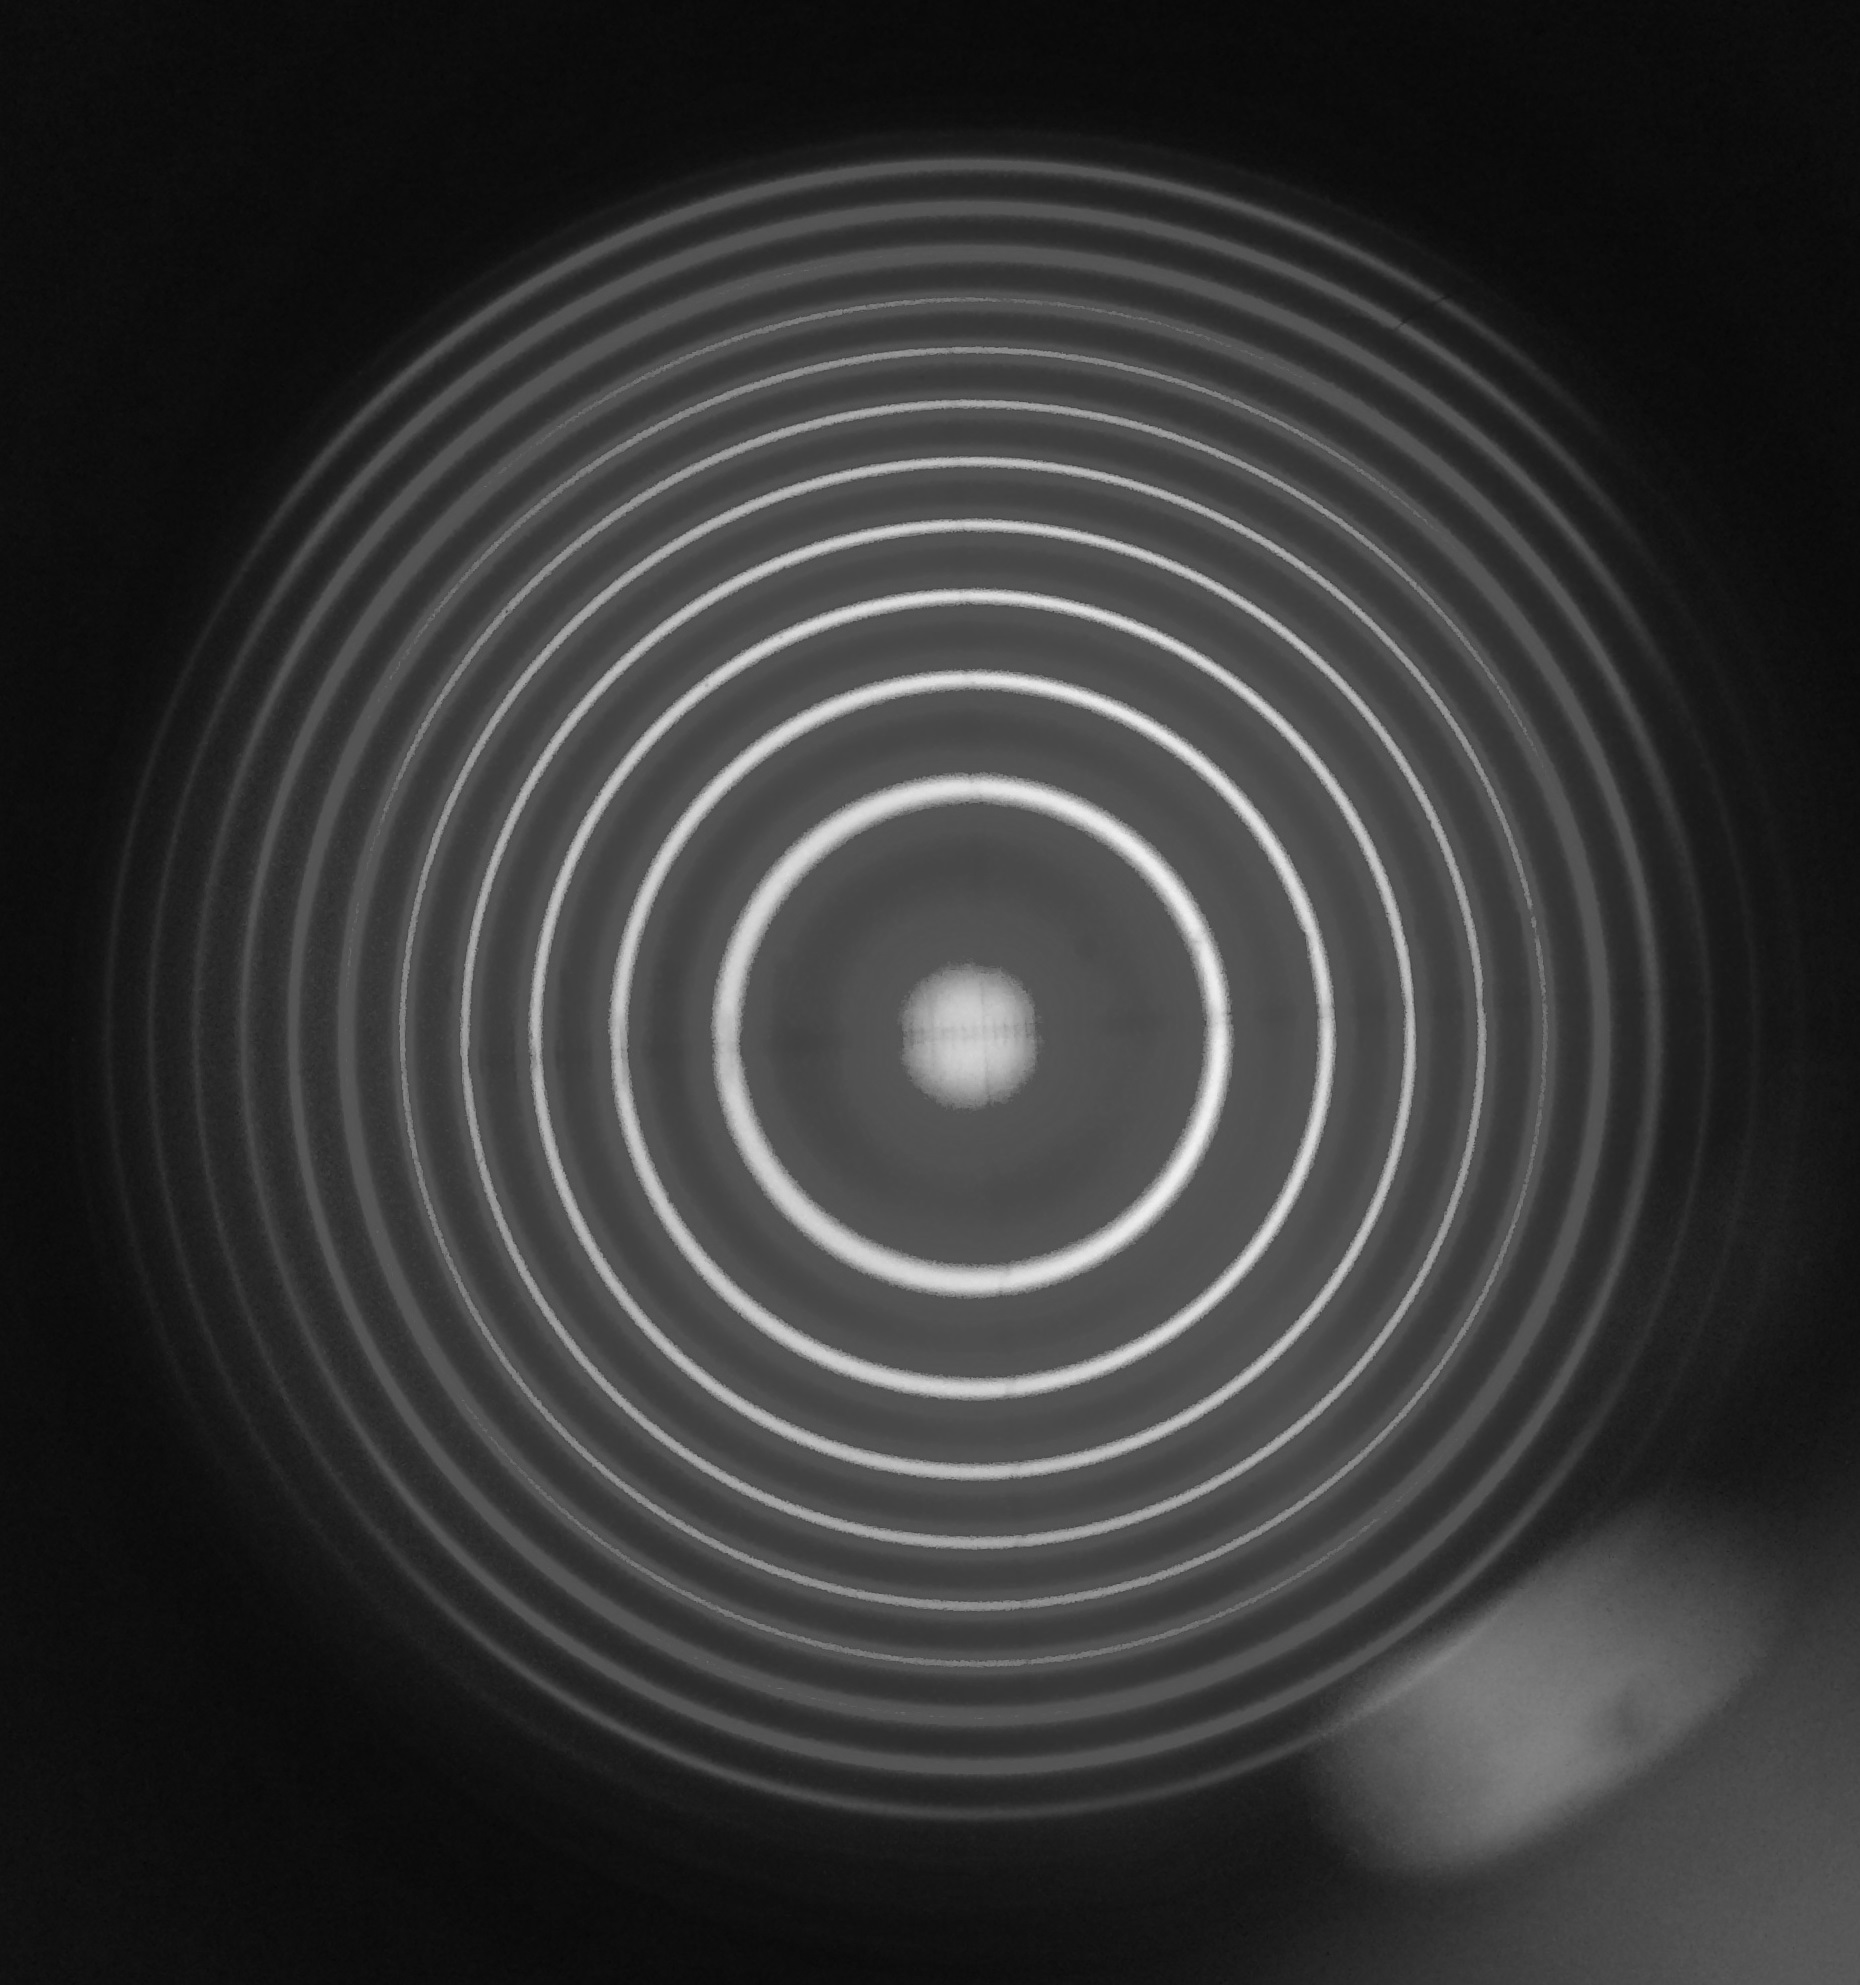
\includegraphics[scale=0.1]{data/bilder_okular/bild_1_edit.jpg}
\caption{Interferenzmuster ohne Magnetfeld}
\label{fig:bildtransohneB}
\end{figure}
In Abb. \ref{fig:bildtransohneB} ist das Interferenzmuster ohne Magnetfeld dargestellt. Man kann gut die konzentrischen Kreise erkennen.\\
\begin{figure}
\centering
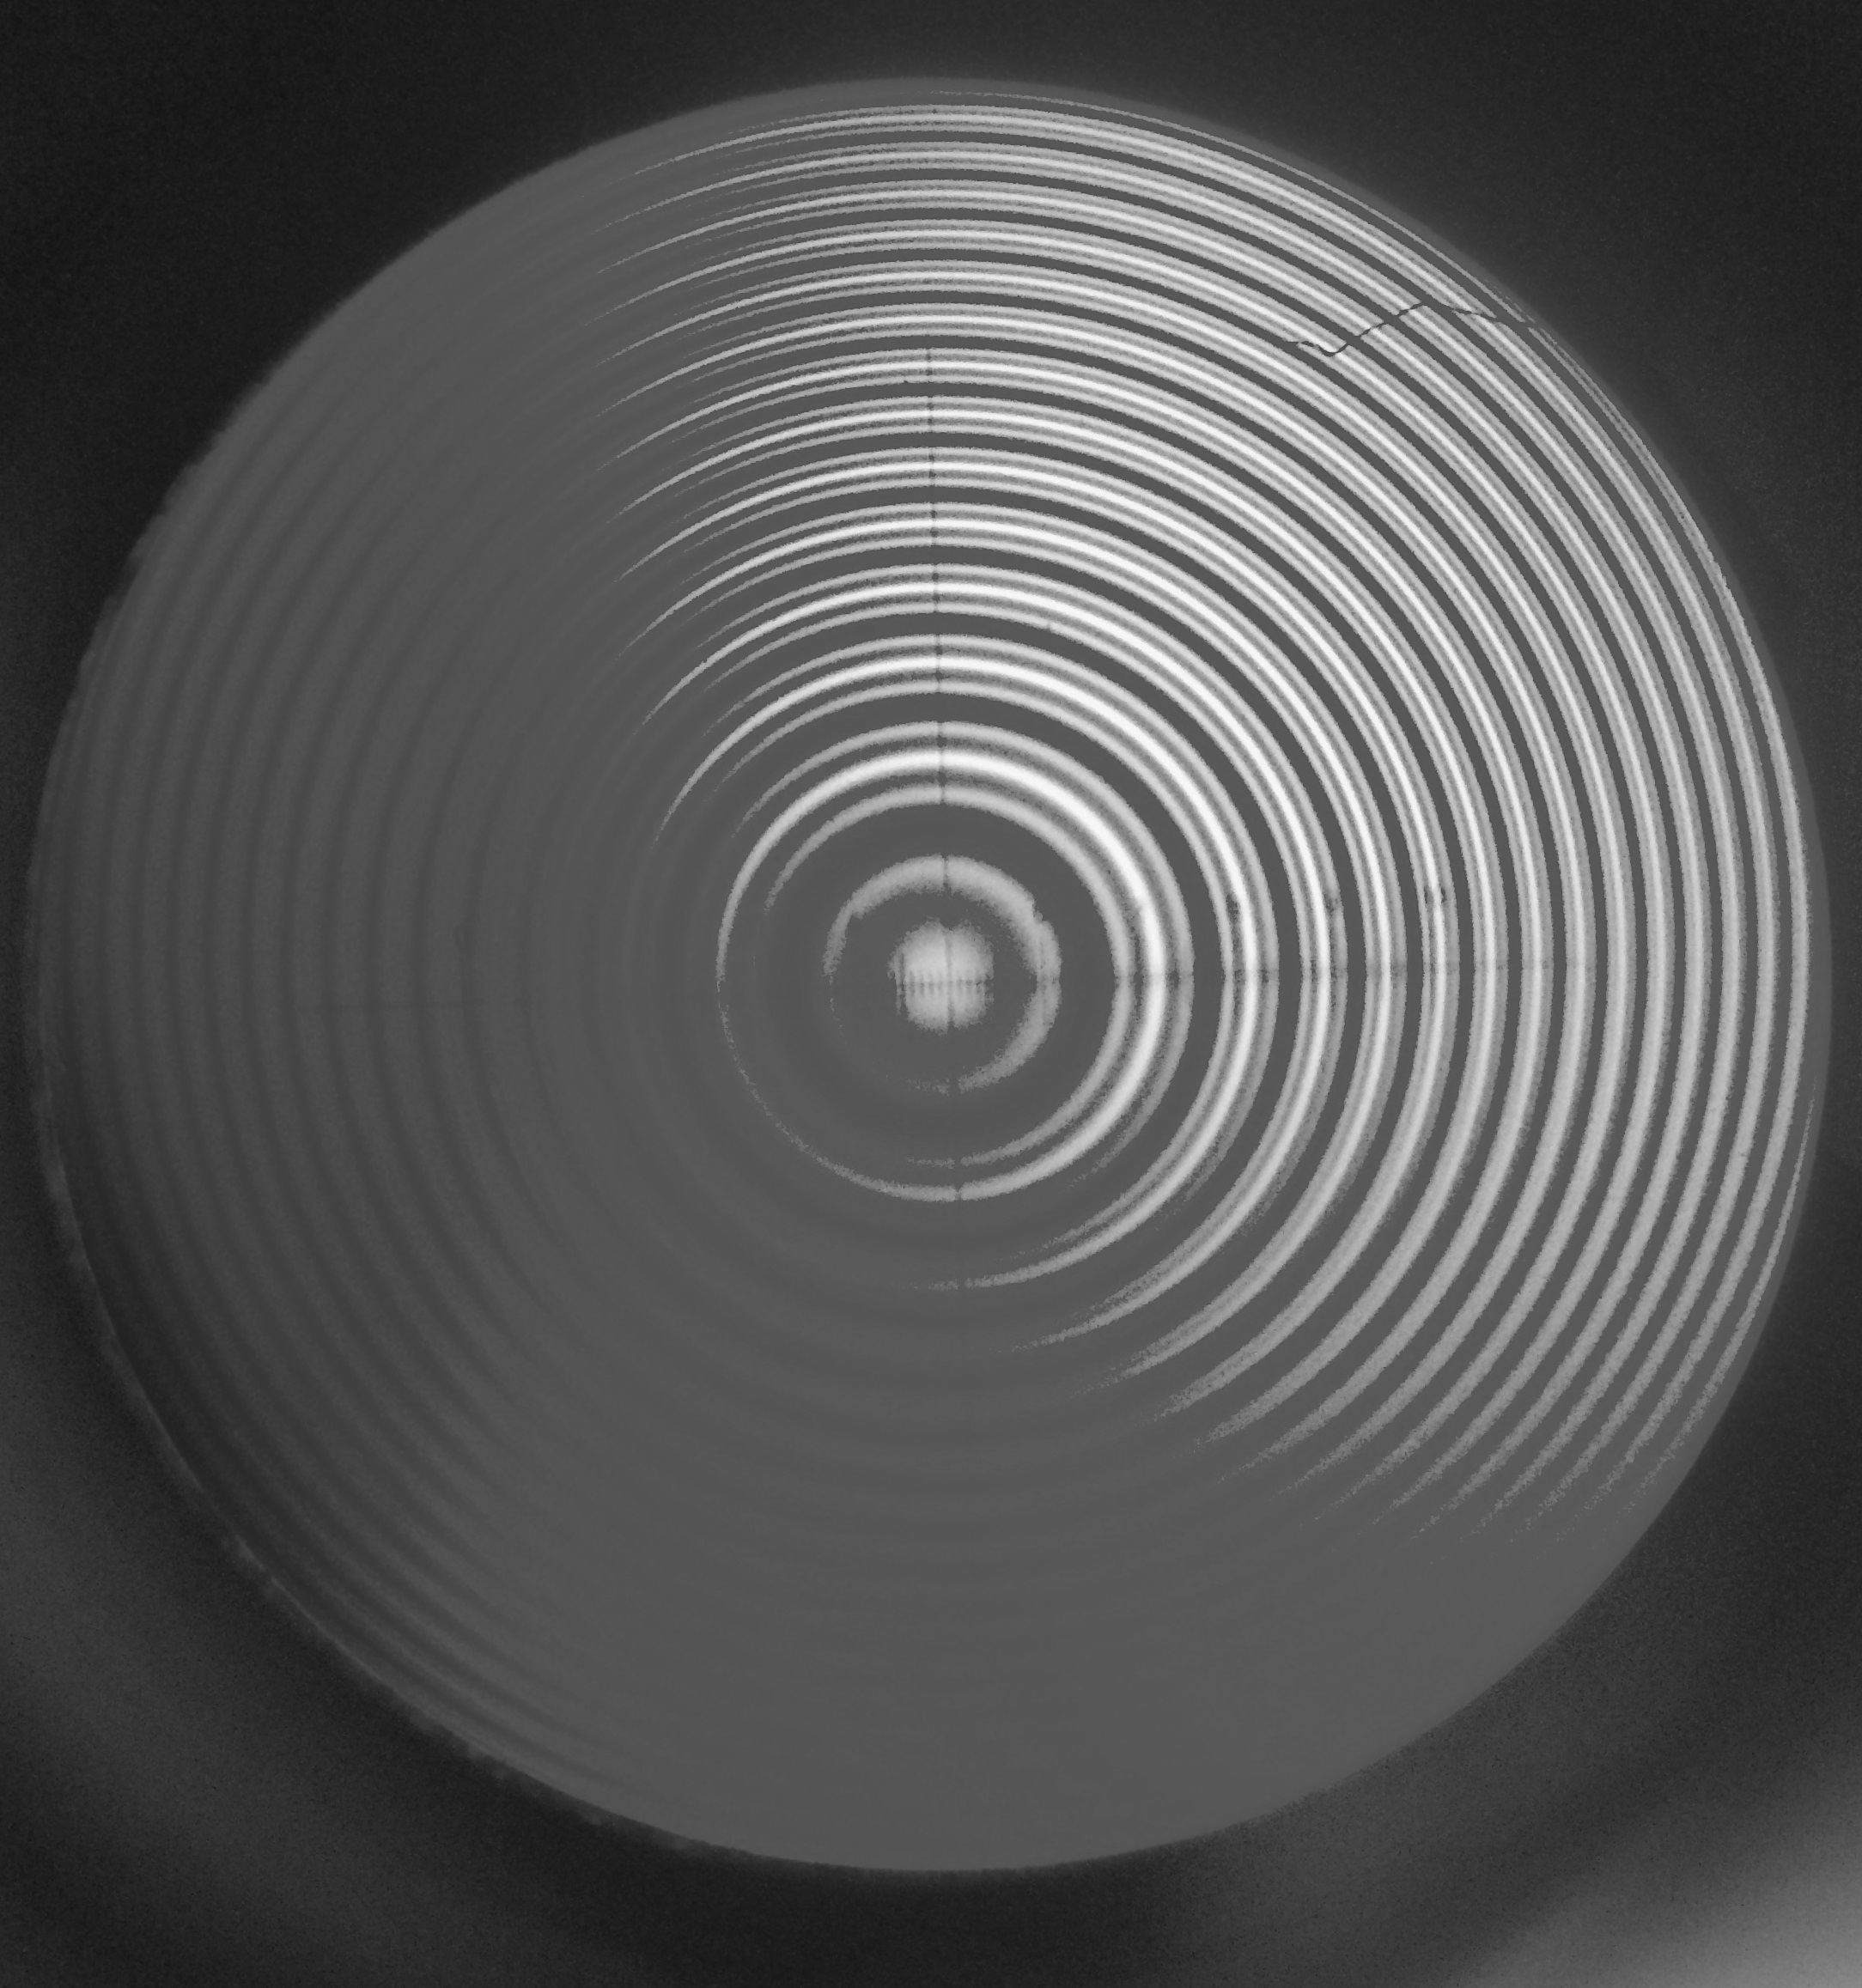
\includegraphics[scale=0.1]{data/bilder_okular/bild_2_edit.jpg}
\caption{Interferenzmuster mit Magnetfeld}
\label{fig:bildtransmitB}
\end{figure}
In Abb. \ref{fig:bildtransmitB} ist das Interferenzmuster mit Magnetfeld dargestellt. Es kommt zu einer Aufspaltung der Kreise in 3 Kreise, wobei die beiden äußeren Kreise schwächer sind.\\
\begin{figure}
\centering
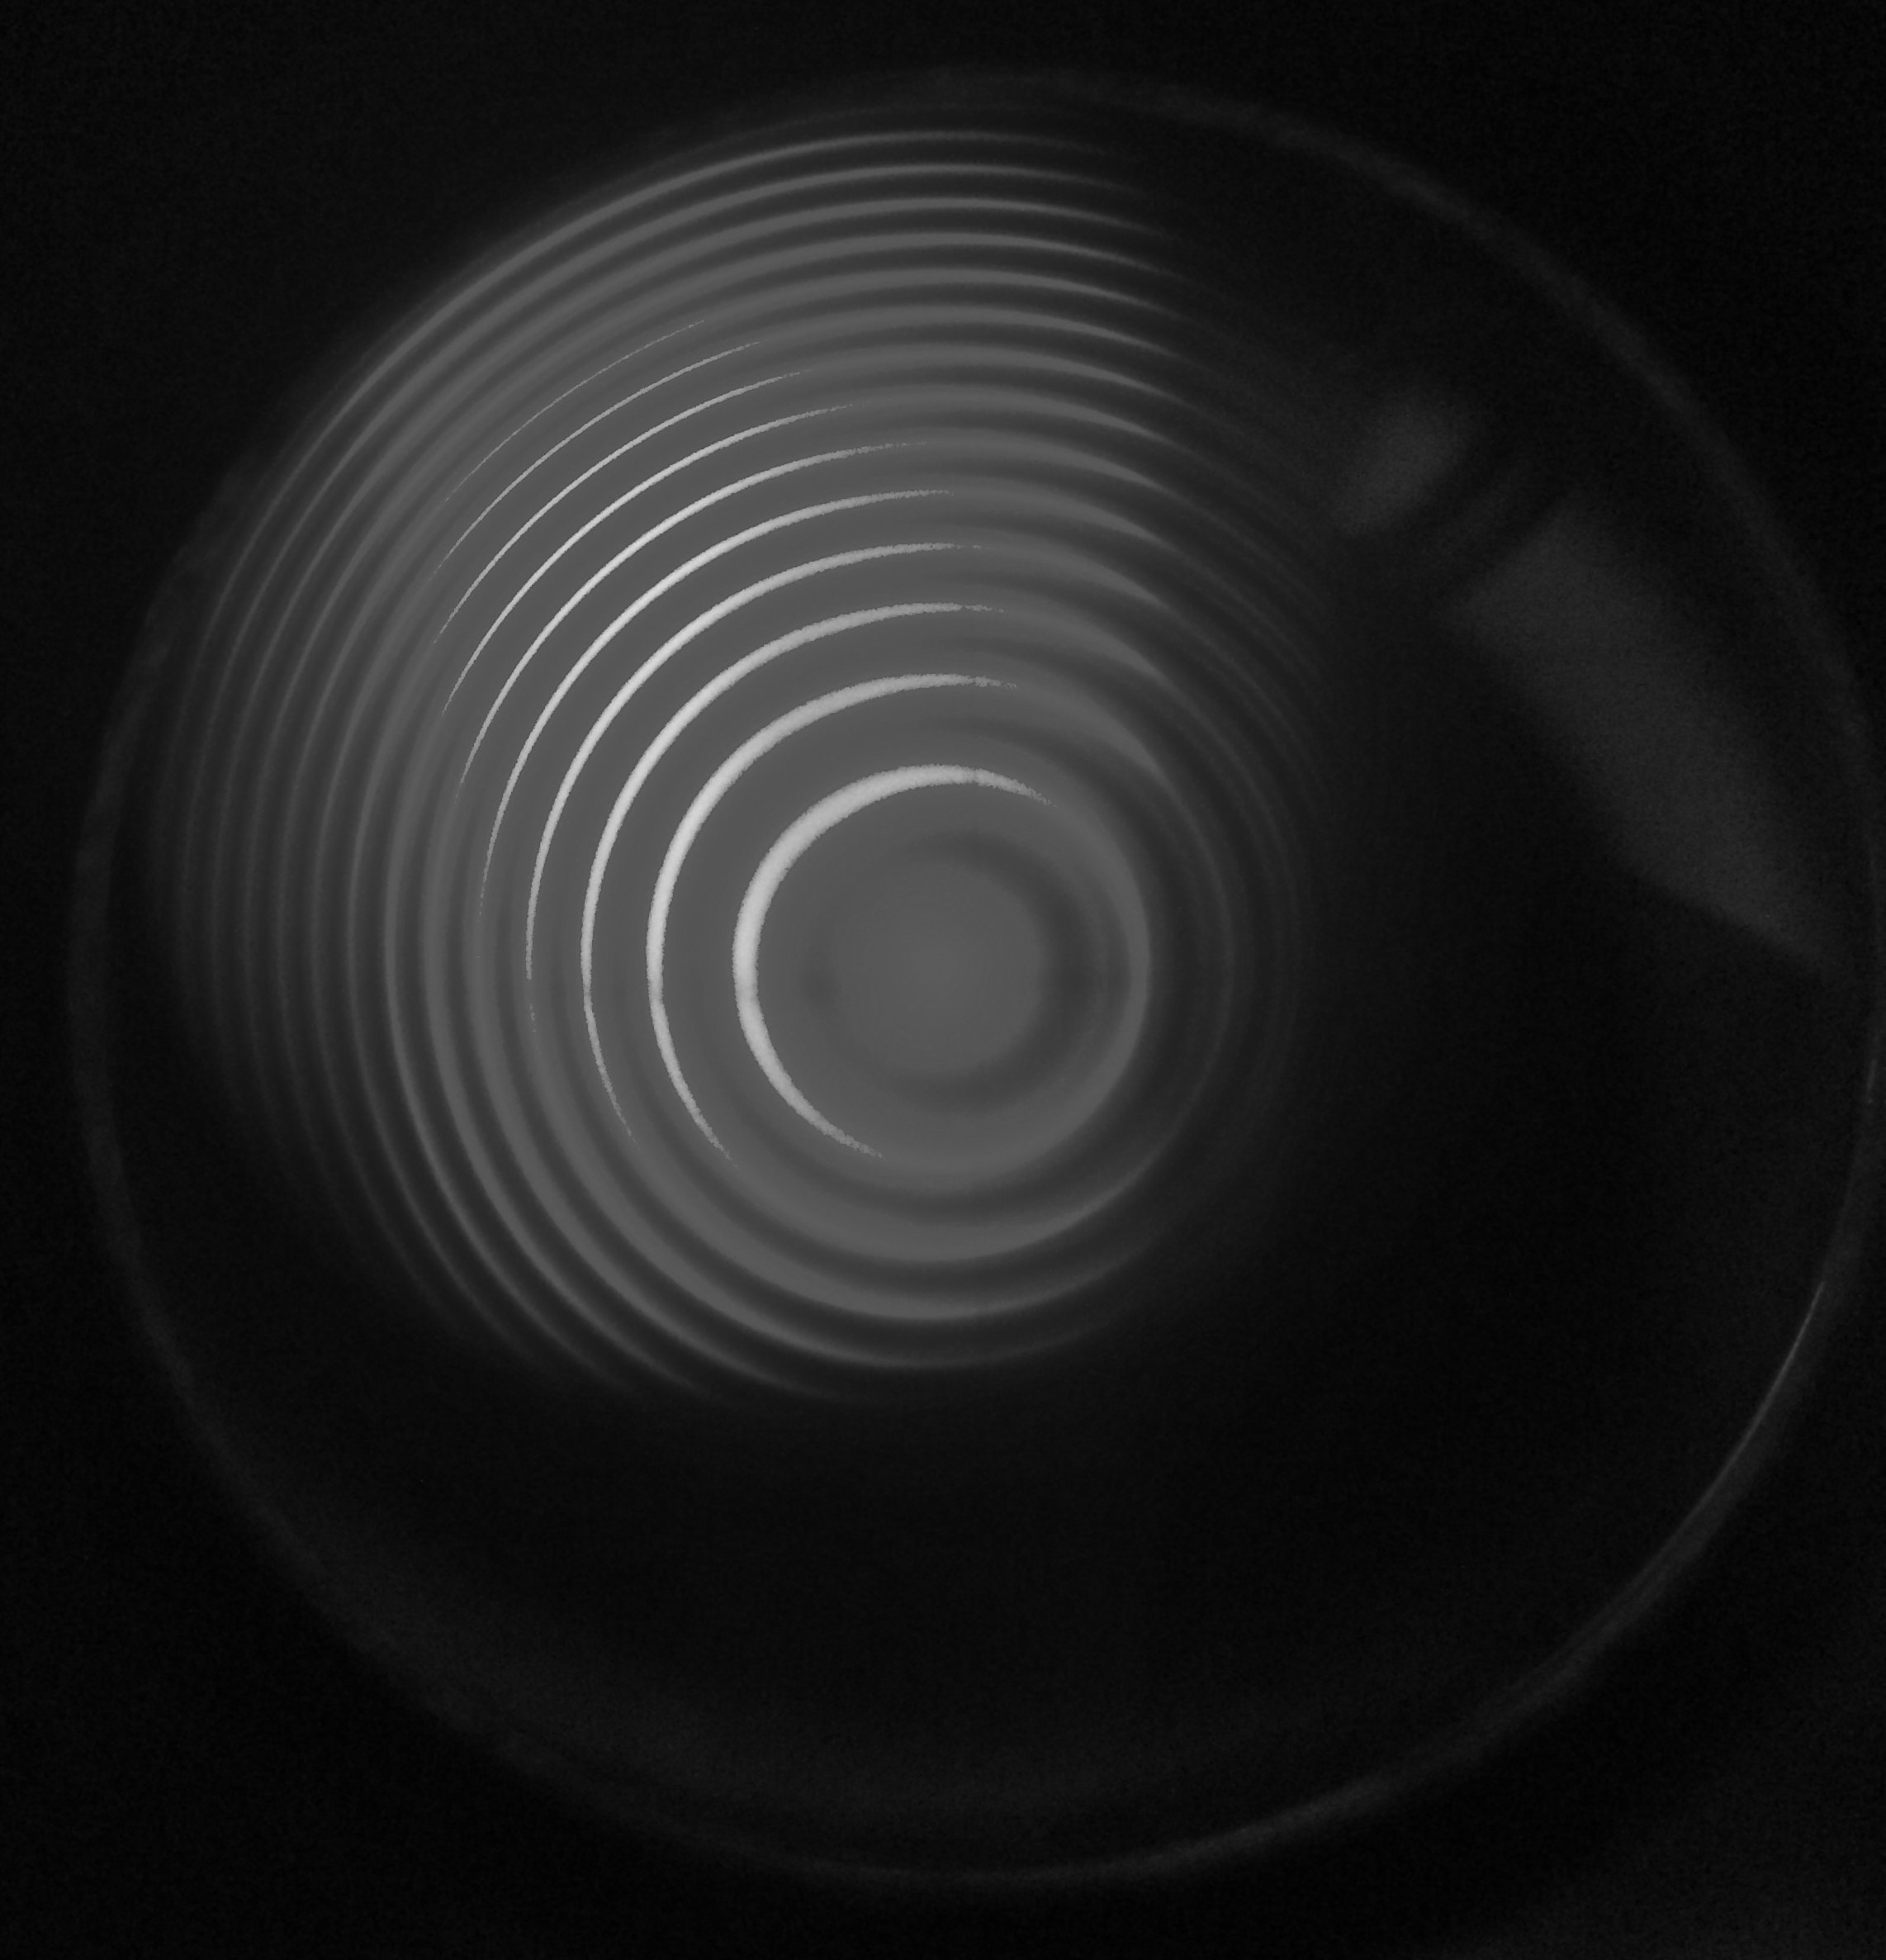
\includegraphics[scale=0.1]{data/bilder_okular/bild_3_edit.jpg}
\caption{Interferenzmuster mit Magnetfeld ohne $\sigma$-Komponenten}
\label{fig:bildtransmitBsigma}
\end{figure}
Stellt man einen Polarisationsfilter vor das Okular, so verschwinden unter dem Winkel von etwa $0^\circ$ zur Magnetfeldachse die $\sigma$-Komponenten (siehe Abb. \ref{fig:bildtransmitBsigma}) und unter dem Winkel von $90^\circ$ die $\pi$-Komponente (siehe Abb. \ref{fig:bildtransmitBpi}).\\
\begin{figure}
\centering
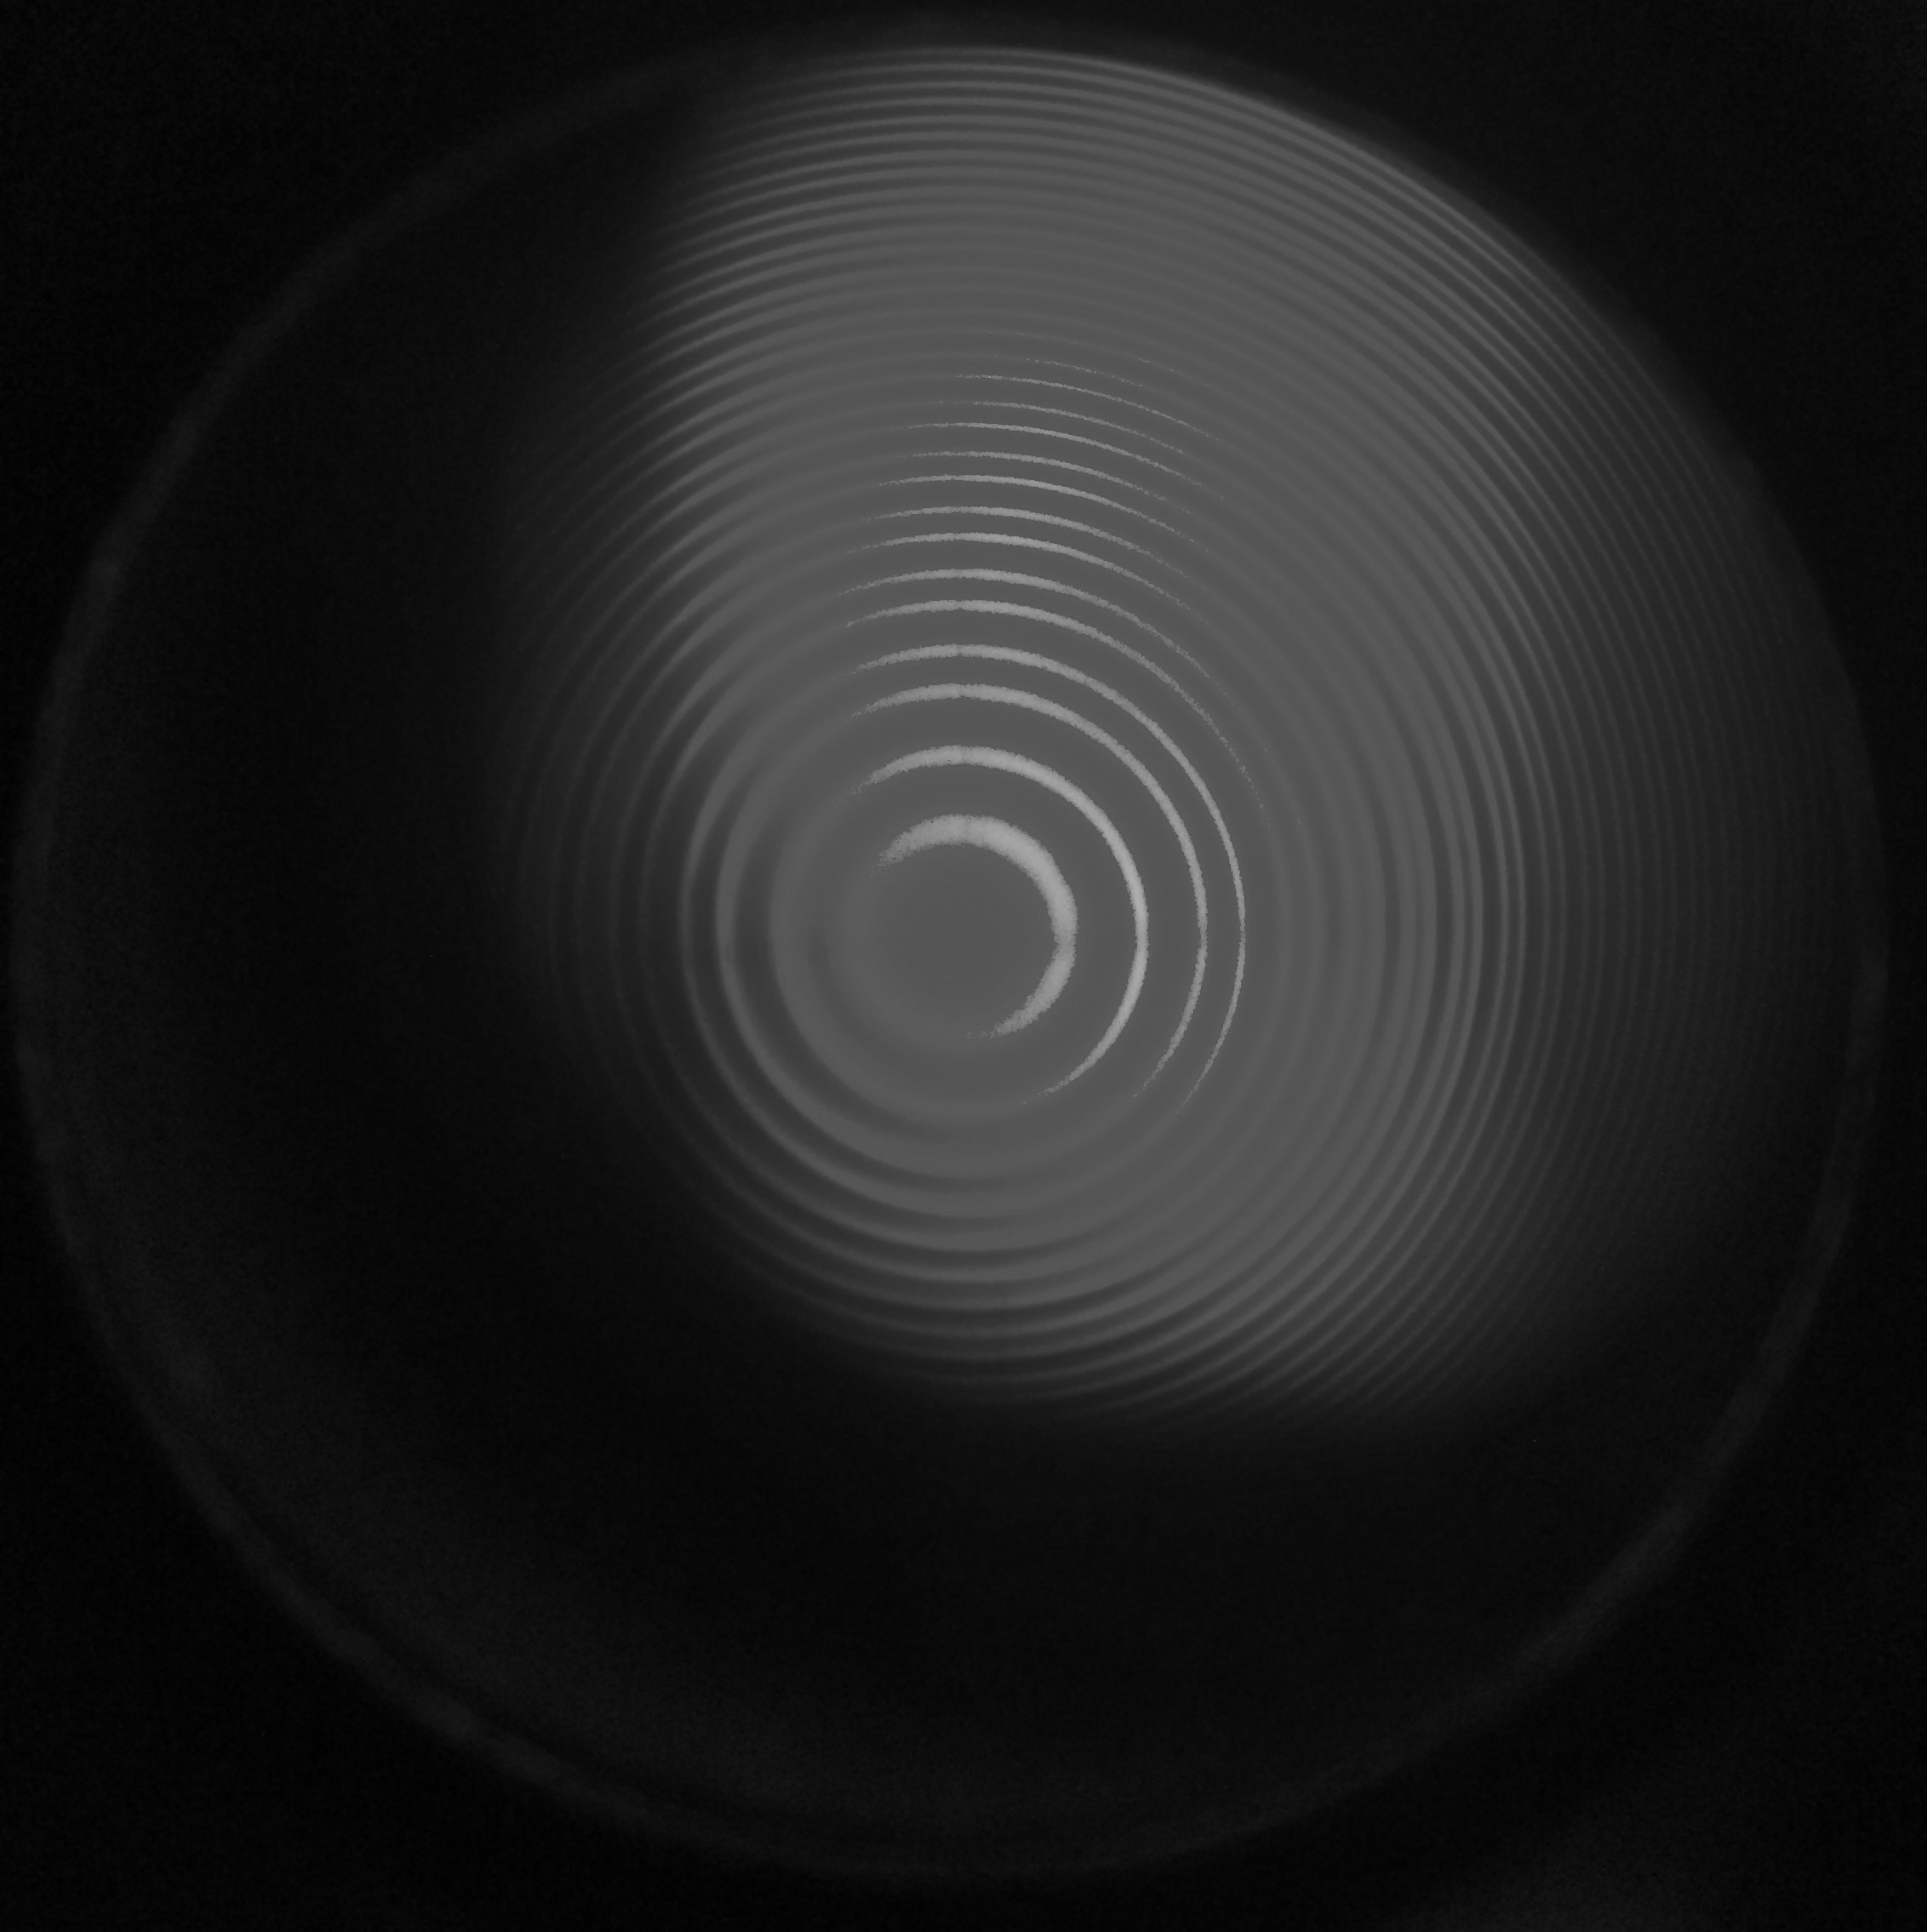
\includegraphics[scale=0.1]{data/bilder_okular/bild_4_edit.jpg}
\caption{Interferenzmuster mit Magnetfeld ohne $\pi$-Komponente}
\label{fig:bildtransmitBpi}
\end{figure}
Bei einem Strom von $\si{(1,8\pm 0,1)\ampere}$ kann man die Linien gerade noch trennen.

\subsubsection{Longitudinale Konfiguration}
\begin{figure}
\centering
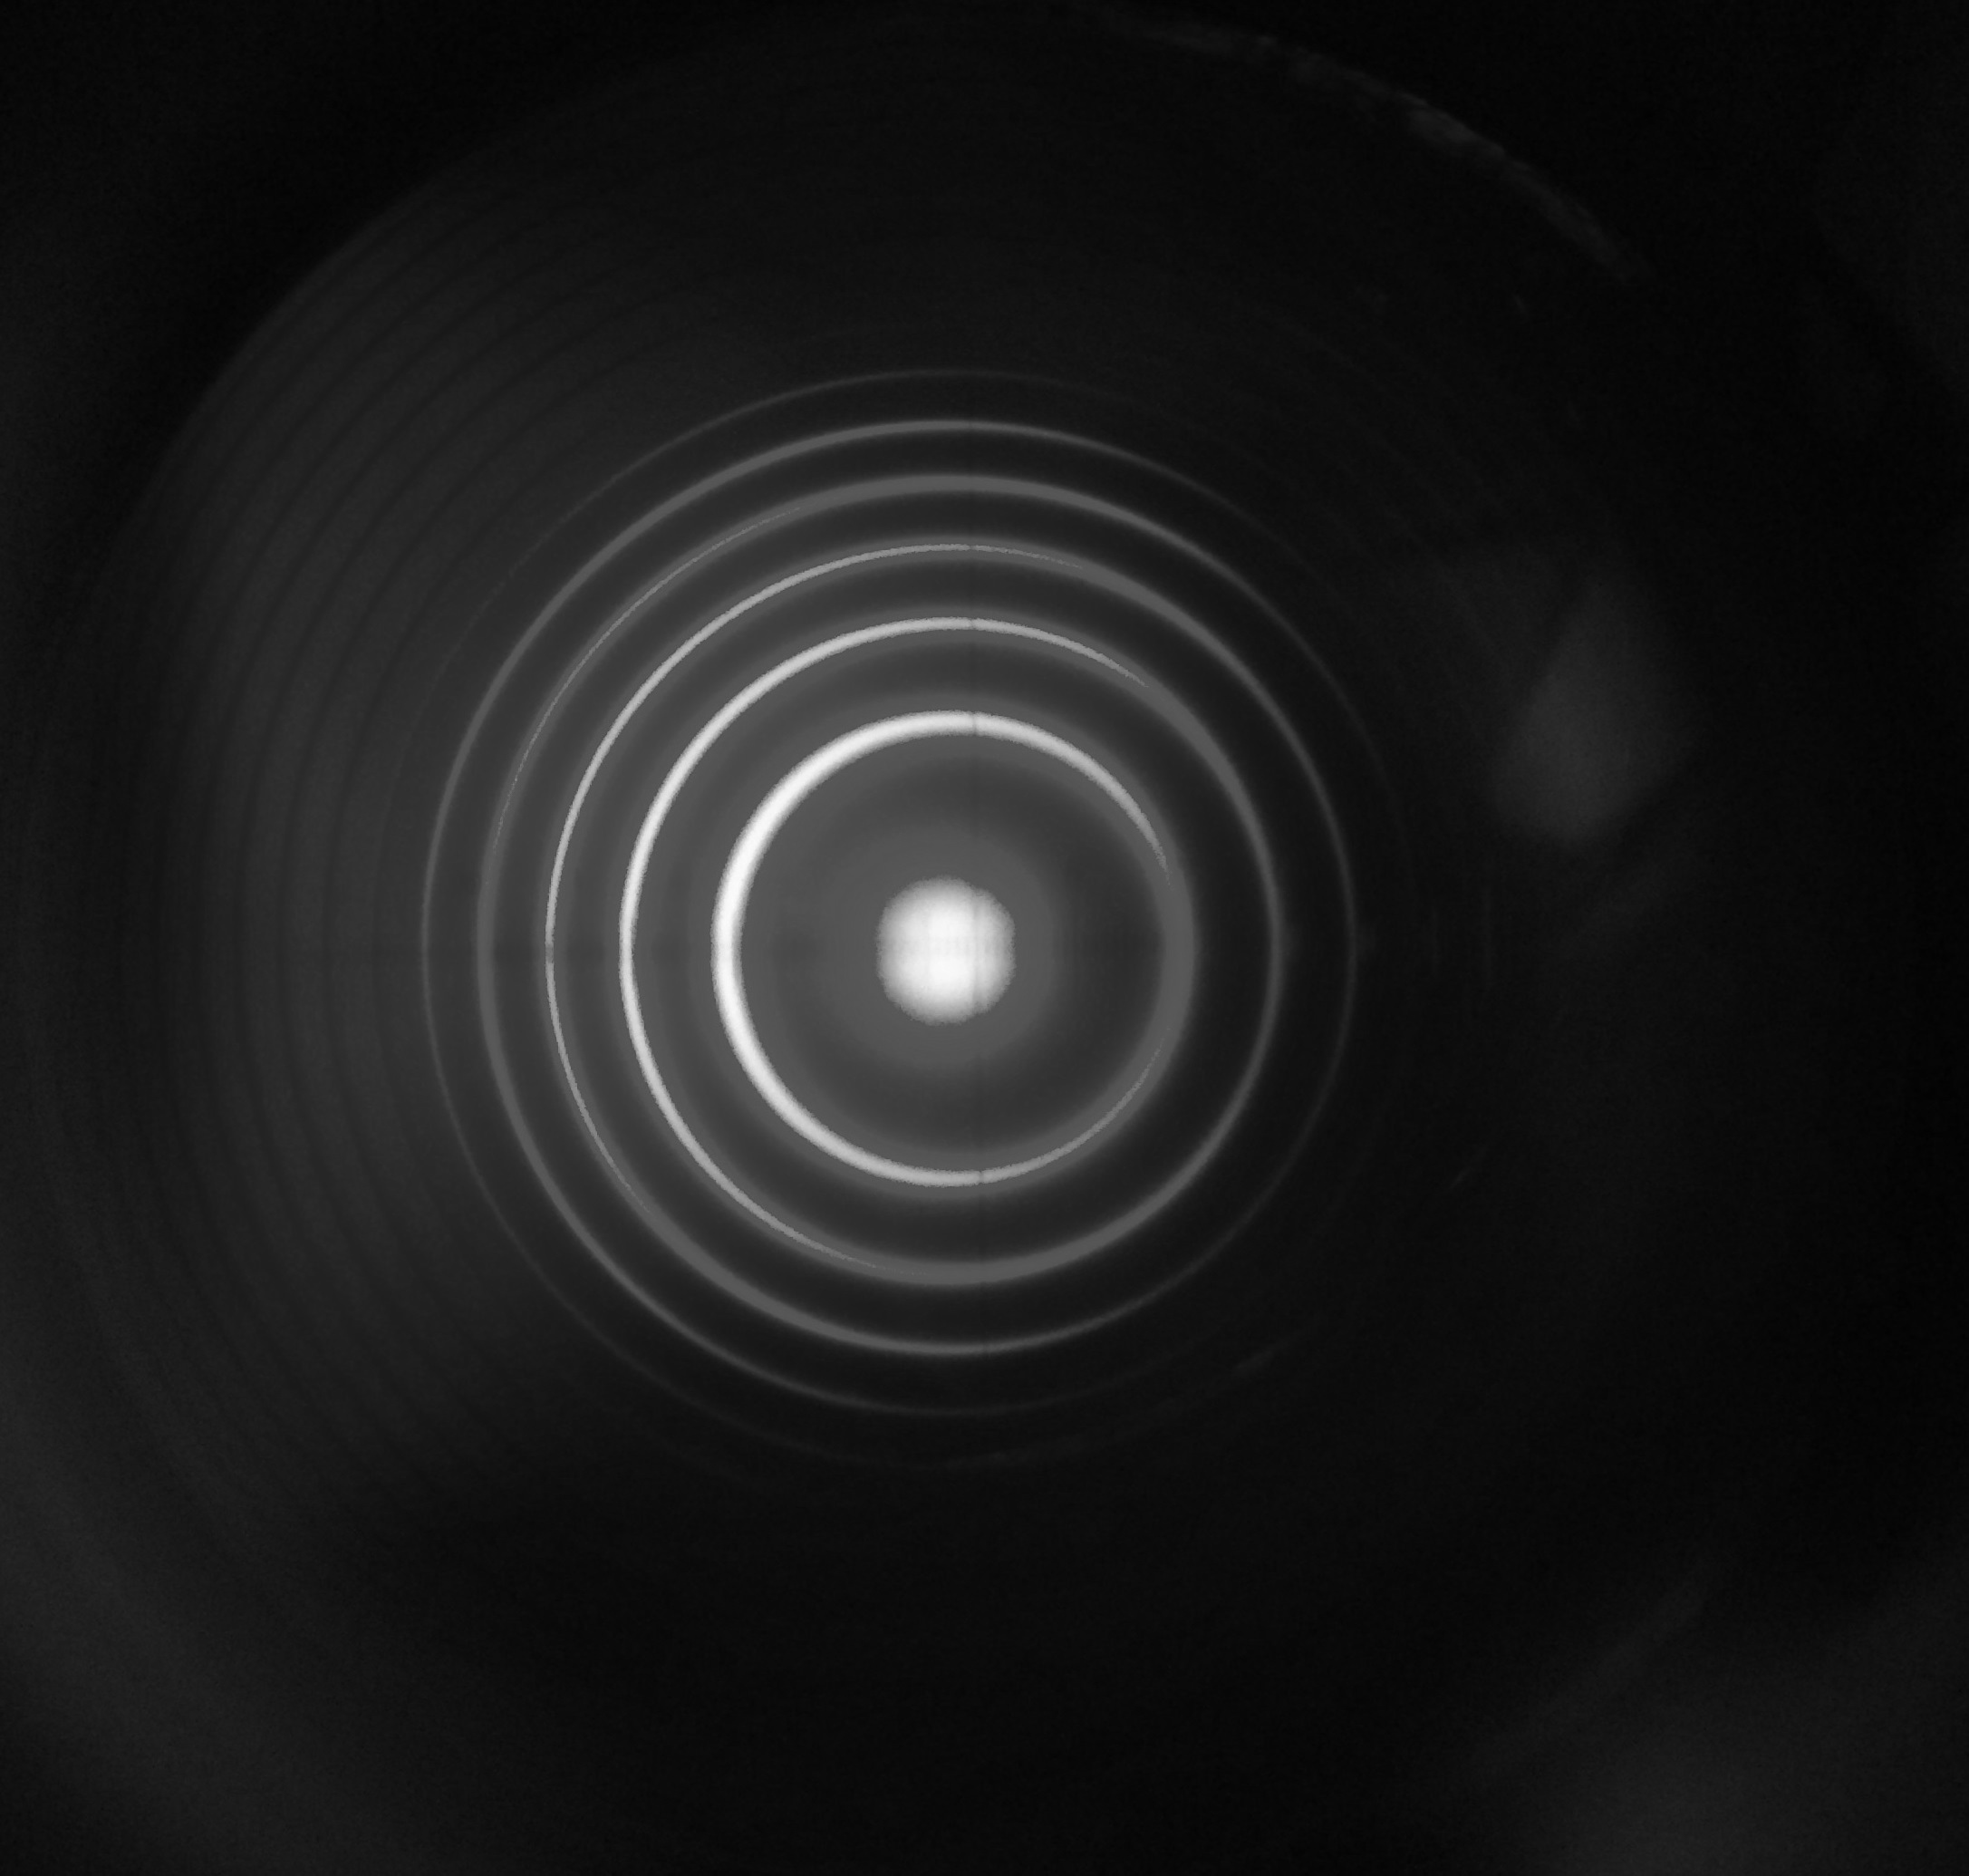
\includegraphics[scale=0.1]{data/bilder_okular/bild_5_edit.jpg}
\caption{Interferenzmuster ohne Magnetfeld}
\label{fig:bildlongohneB}
\end{figure}
Betrachtet man das Interferenzmuster in longitudinaler Richtung, also in Richtung des Magnetfeldes, so ist ohne Magnetfeld (siehe Abb. \ref{fig:bildlongohneB}) kein Unterschied zu erkennen. Wenn man das Magnetfeld hochfährt (siehe Abb. \ref{fig:bildlongmitB}) spalten sich die Linien wieder auf. Allerdings sind diesmal nur 2 Kreise zu sehen, der mittlere fehlt.
\begin{figure}
\centering
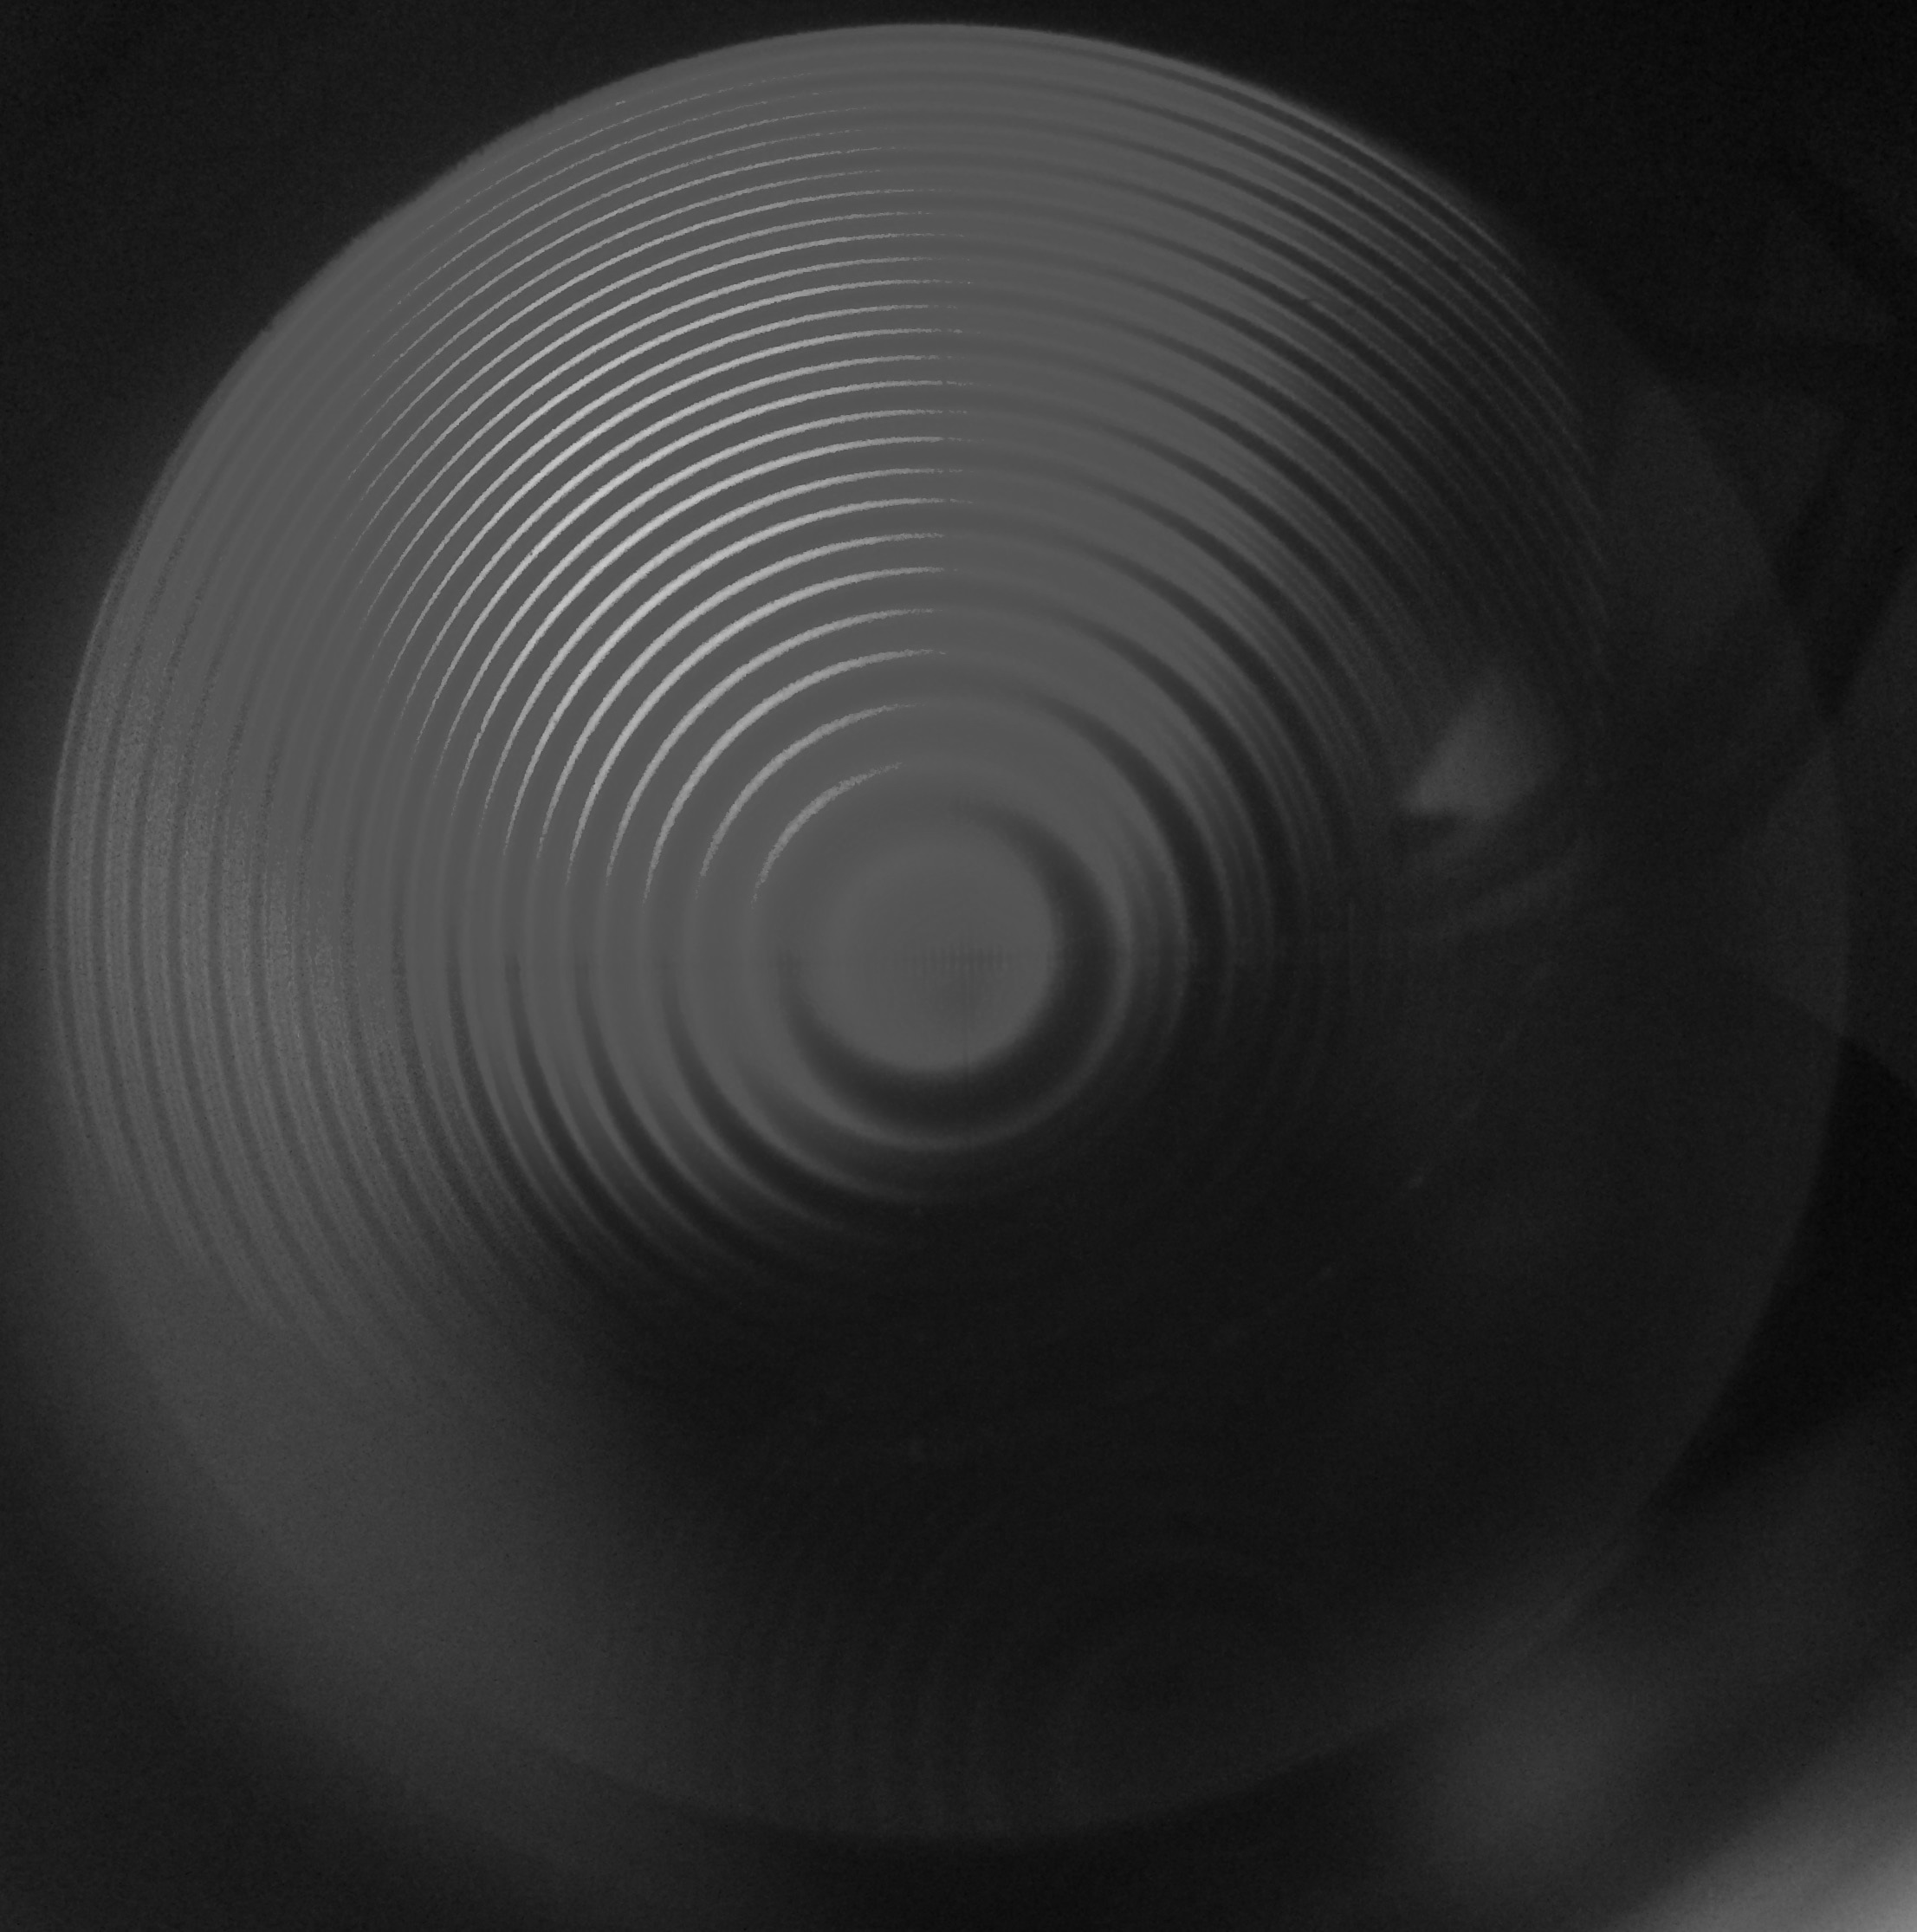
\includegraphics[scale=0.1]{data/bilder_okular/bild_6_edit.jpg}
\caption{Interferenzmuster mit Magnetfeld}
\label{fig:bildlongmitB}
\end{figure}
\begin{figure}
\centering
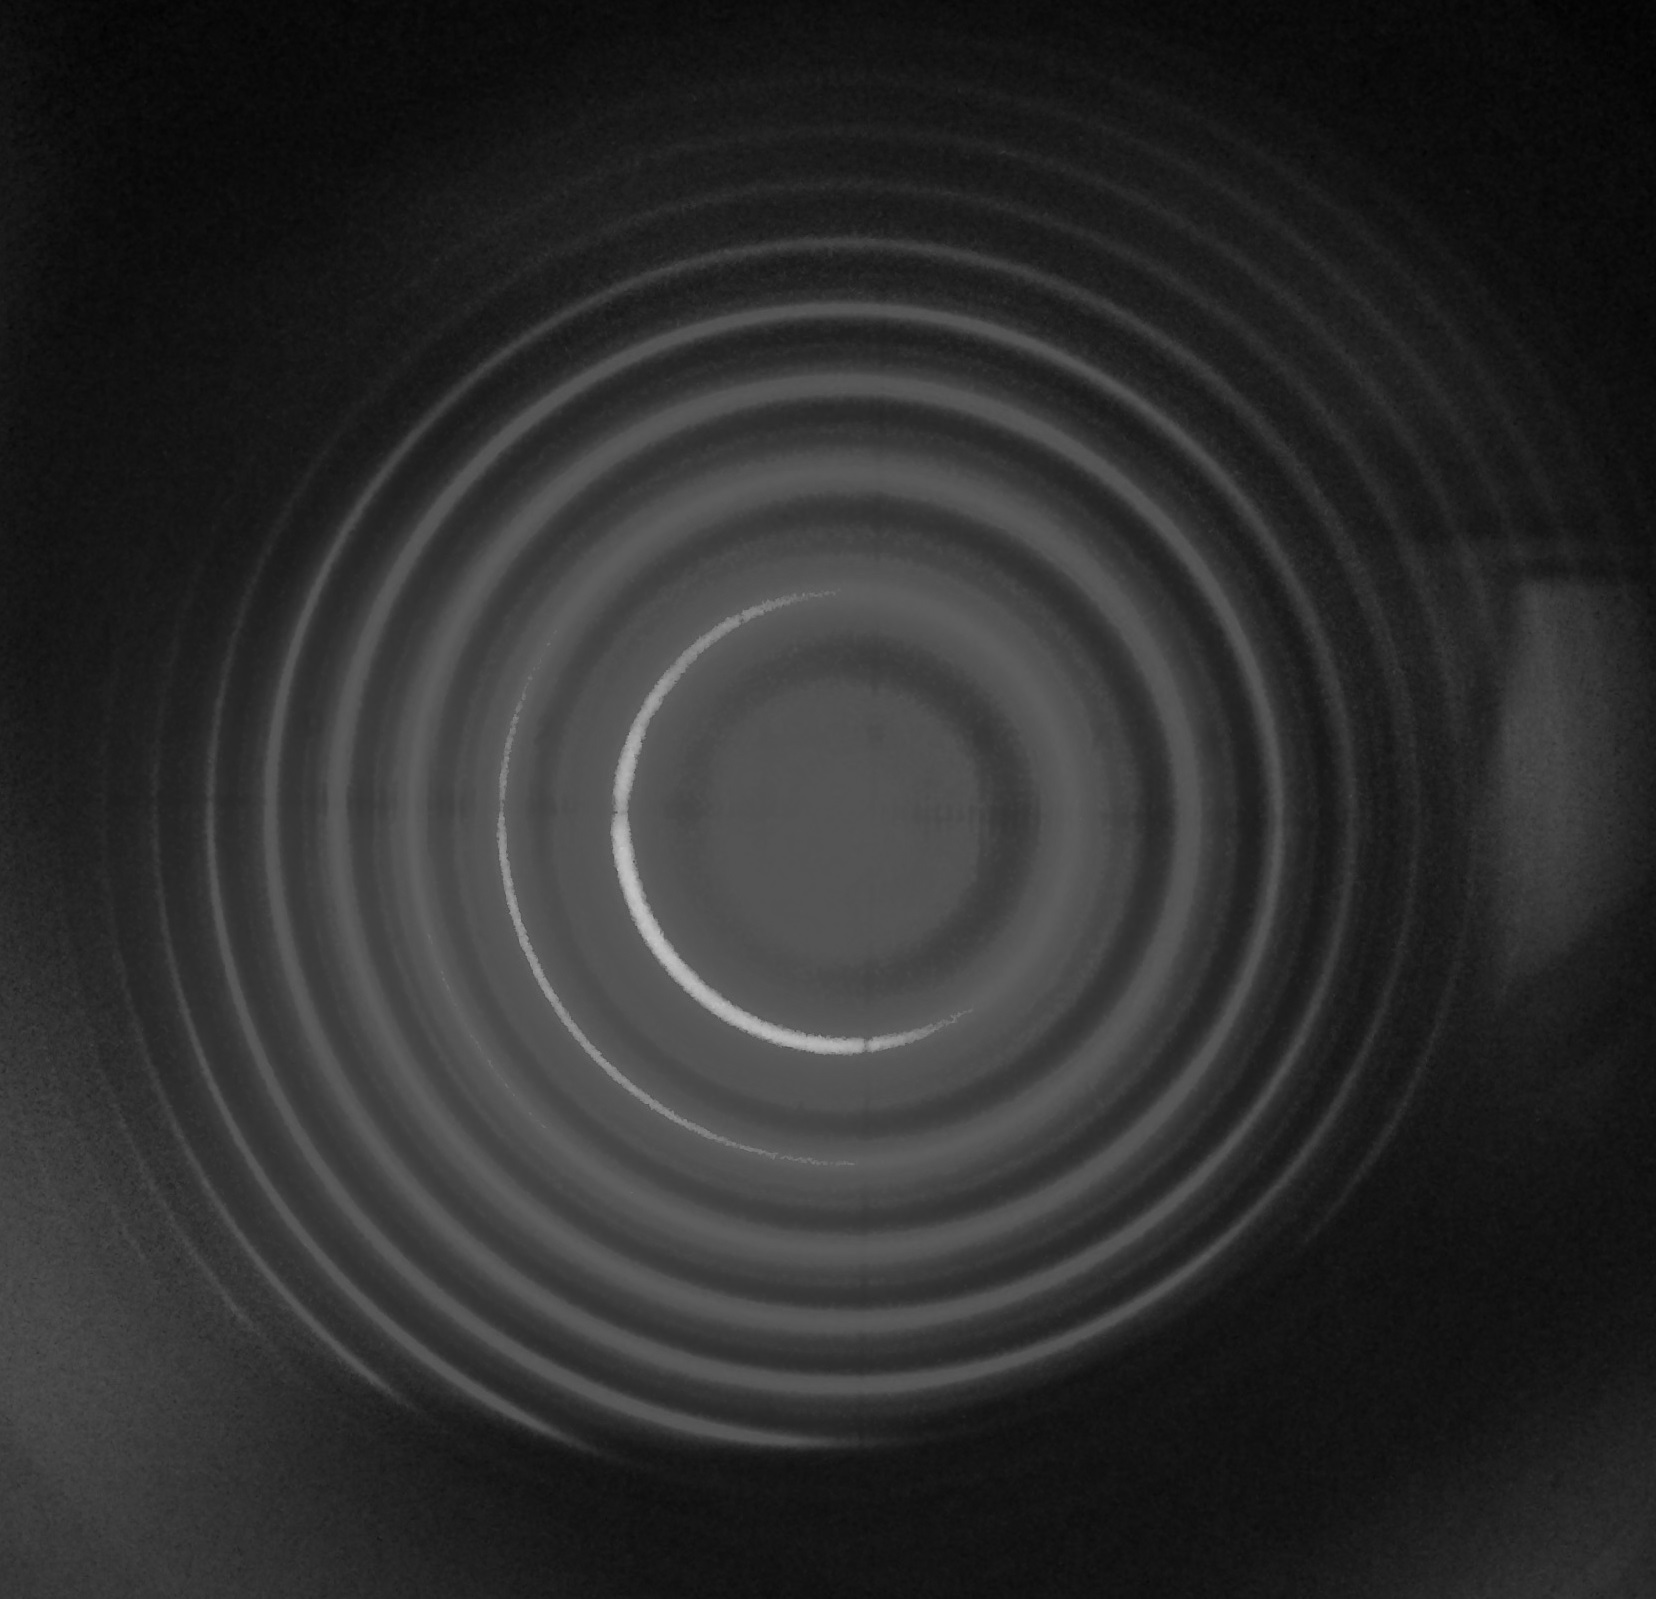
\includegraphics[scale=0.1]{data/bilder_okular/bild_7_edit.jpg}
\caption{Interferenzmuster mit Magnetfeld ohne $\sigma^+$-Komponente}
\label{fig:bildlongmitBsigmaplus}
\end{figure}
Stellt man ein $\lambda/4$-Plättchen und einen Polarisationsfilter vor das Okular, so verschwinden unter dem Winkel von etwa $(-44 \pm 5)^\circ$ zur optischen Achse des $\lambda/4$-Plättchens die äußere ($\sigma^+$) Komponente (siehe Abb. \ref{fig:bildlongmitBsigmaplus}) und unter einem Winkel von $(43 \pm 5)^\circ$ die innere ($\sigma^-$) Komponente (siehe Abb. \ref{fig:bildlongmitBsigmaminus}). Beides ist in den Abbildungen leider nicht sehr gut zu erkennen.\\
\begin{figure}
\centering
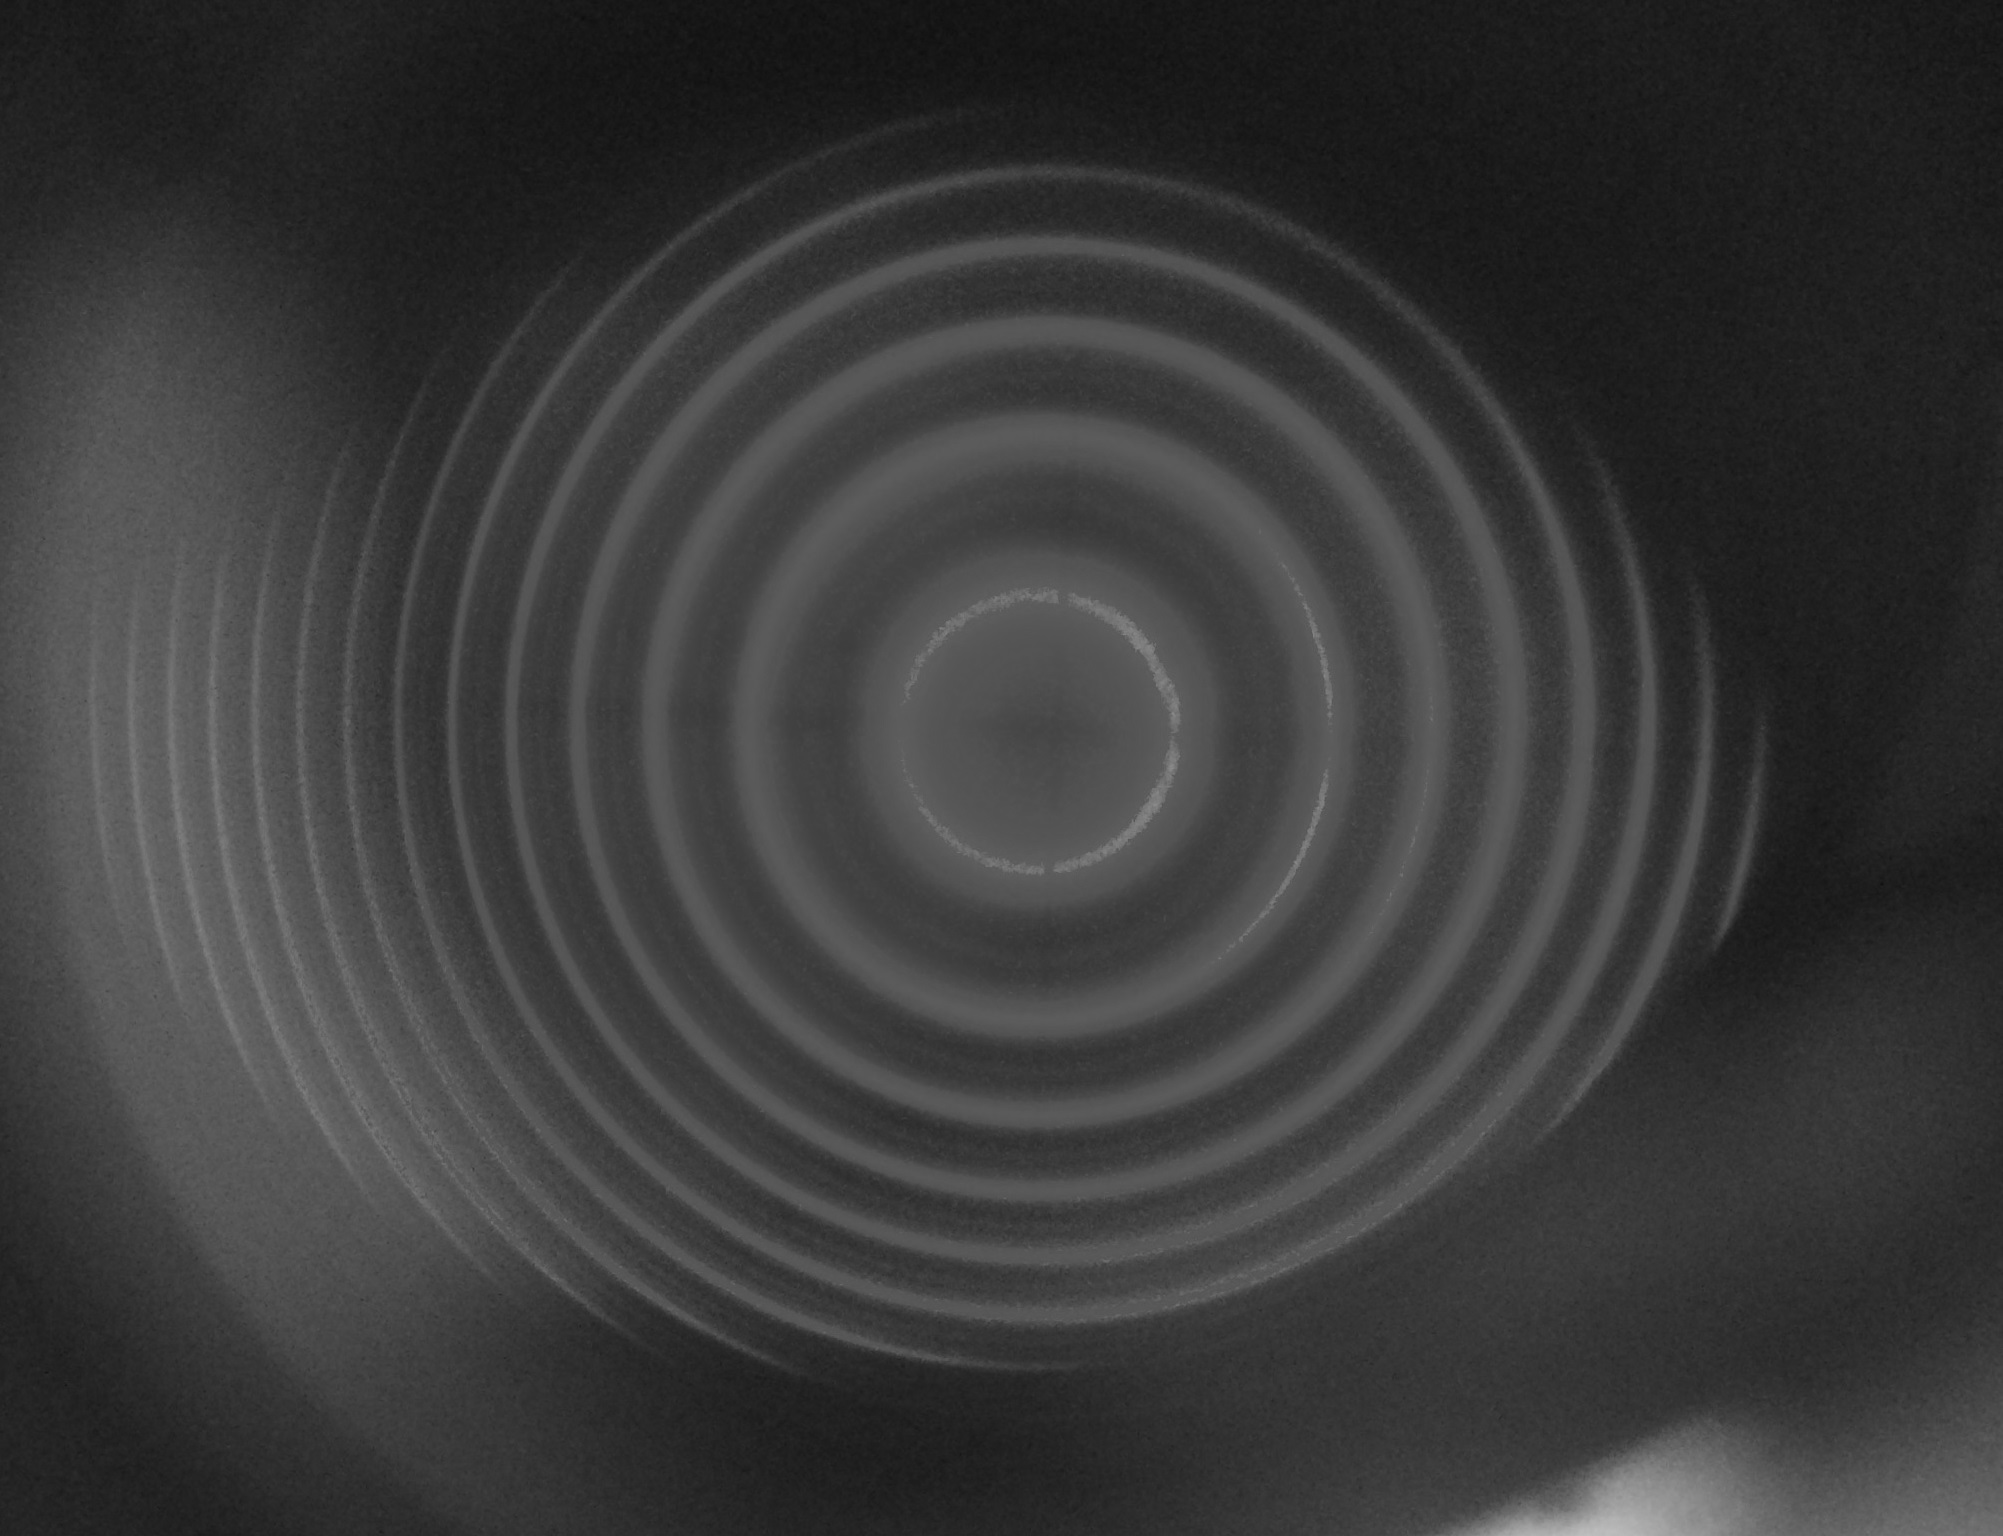
\includegraphics[scale=0.1]{data/bilder_okular/bild_8_edit.jpg}
\caption{Interferenzmuster mit Magnetfeld ohne $\sigma^-$-Komponente}
\label{fig:bildlongmitBsigmaminus}
\end{figure}
Bei einem Strom von $\si{(1,1\pm 0,1)\ampere}$ kann man die Linien gerade noch trennen.